% SC4022 --- Chapter 4: Random Graphs (ER, Configuration, Small-World) (0->100 ground-up)
\chapter{Random Graphs: Erd\H{o}s--R\'enyi, Configuration \& Small-World}
\label{ch:random}
\sloppy

\begin{quote}
\emph{``What does a typical network look like?''} --- If you toss a coin for every possible edge, what graph appears? When does it become connected? How can we build a random graph with a prescribed degree sequence, or one that is both clustered and short?
\end{quote}

\noindent\fbox{\parbox{\dimexpr\linewidth-2\fboxsep-2\fboxrule}{%
\textbf{From zero: we build here, no random-graph background needed.} We assume only Ch.~1 (graph, degree, clustering, path) and basic probability (SC2000: Bernoulli, binomial, expectation). Every model is motivated by a picture, then defined, then exercised.}}
\vspace{0.4em}

\section*{Learning Outcomes}
After this chapter you will be able to:
\begin{enumerate}[label=(L\arabic*)]
    \item define $G(n,p)$ and $G(n,M)$, derive degree distribution and $\langle k\rangle$;
    \item explain the giant-component phase transition at $p=1/n$ (or $\langle k\rangle=1$);
    \item construct the configuration model and generate graphs with arbitrary $P(k)$;
    \item generate Watts--Strogatz small-world graphs and quantify the clustering vs path trade-off;
    \item test whether a real network's feature is significant against a null (random) model.
\end{enumerate}

% ============================================================
\section{Erd\H{o}s--R\'enyi: $G(n,p)$ and $G(n,M)$}
\label{sec:er}
\paragraph{Intuition.} Flip a biased coin with heads probability $p$ for each of the $\binom{n}{2}$ possible undirected edges, independently. Heads = keep the edge. The resulting graph is random, yet its typical properties are sharply predictable: for tiny $p$ it is dust (isolated nodes); as $p$ grows, a giant connected piece suddenly appears, then the whole graph connects.

\begin{definition}[Erd\H{o}s--R\'enyi models]\label{def:er}
$G(n,p)$: $n$ labelled nodes, each edge present independently with probability $p$. $G(n,M)$: uniform over all graphs with exactly $M$ edges ($0\le M\le\binom{n}{2}$). They are asymptotically equivalent when $M=p\binom{n}{2}$ and $n$ large.
\end{definition}

\paragraph{Degree distribution.} Fix a node $v$; its degree $k_v\sim\text{Binomial}(n-1,p)$ because each of the $n-1$ potential neighbours is present with prob.\ $p$:
\begin{equation}
\Pr(k_v=k)=\binom{n-1}{k}p^k(1-p)^{\,n-1-k},\quad \langle k\rangle=(n-1)p\approx np.
\end{equation}
For sparse graphs with $\langle k\rangle$ fixed and $n\to\infty$, $p=\langle k\rangle/n$ and the binomial tends to Poisson($\langle k\rangle$):
\begin{equation}
P(k)\approx e^{-\langle k\rangle}\langle k\rangle^k/k!.
\end{equation}
So ER degrees are concentrated near the mean, unlike the heavy tails of Ch.~5.

\begin{figure}[h]\centering
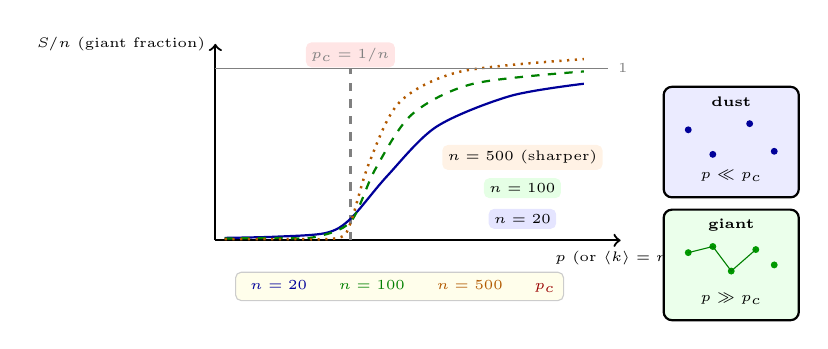
\begin{tikzpicture}[scale=0.78,every node/.style={font=\scriptsize}]
% giant component S-curve
\draw[->,thick] (0,0)--(6.6,0) node[below,font=\tiny] {$p$ (or $\langle k\rangle=np$)};
\draw[->,thick] (0,0)--(0,3.2) node[left,font=\tiny] {$S/n$ (giant fraction)};
\draw[dashed,gray,thick] (2.2,0)--(2.2,2.8) node[above,font=\tiny,fill=red!10,rounded corners=2pt,inner sep=2pt] {$p_c=1/n$};
\draw[thick,blue!60!black,smooth] plot coordinates {(0.15,0.04) (1.0,0.06) (1.8,0.12) (2.2,0.35) (2.8,1.05) (3.6,1.85) (4.8,2.35) (6.0,2.55)};
\draw[thick,green!50!black,smooth,dashed] plot coordinates {(0.15,0.03) (1.0,0.04) (1.6,0.05) (2.2,0.30) (2.6,1.15) (3.2,2.05) (4.2,2.55) (6.0,2.75)};
\draw[thick,orange!70!black,smooth,dotted,line width=0.9pt] plot coordinates {(0.15,0.02) (1.2,0.02) (2.0,0.04) (2.2,0.28) (2.5,1.25) (3.0,2.25) (4.0,2.75) (6.0,2.95)};
\draw[thin,gray] (0,2.8)--(6.4,2.8) node[right,font=\tiny] {1};
\node[font=\tiny,fill=blue!10,rounded corners=2pt,inner sep=2pt] at (5.0,0.35) {$n=20$};
\node[font=\tiny,fill=green!10,rounded corners=2pt,inner sep=2pt] at (5.0,0.85) {$n=100$};
\node[font=\tiny,fill=orange!10,rounded corners=2pt,inner sep=2pt] at (5.0,1.35) {$n=500$ (sharper)};
% small insets: below threshold and above
\begin{scope}[xshift=7.4cm,yshift=1.6cm]
\draw[thick,fill=blue!8,rounded corners=3pt] (-0.1,-0.9) rectangle (2.1,0.9);
\node[font=\tiny\bfseries] at (1.0,0.65) {dust};
\foreach \p in {(0.3,0.2),(0.7,-0.2),(1.3,0.3),(1.7,-0.15)} \fill[blue!60!black] \p circle (1.6pt);
\node[font=\tiny] at (1.0,-0.55) {$p\ll p_c$};
\end{scope}
\begin{scope}[xshift=7.4cm,yshift=-0.4cm]
\draw[thick,fill=green!8,rounded corners=3pt] (-0.1,-0.9) rectangle (2.1,0.9);
\node[font=\tiny\bfseries] at (1.0,0.65) {giant};
\foreach \p in {(0.3,0.2),(0.7,0.3),(1.0,-0.1),(1.4,0.25),(1.7,0)} \fill[green!60!black] \p circle (1.6pt);
\draw[thin,green!50!black] (0.3,0.2)--(0.7,0.3)--(1.0,-0.1)--(1.4,0.25);
\node[font=\tiny] at (1.0,-0.55) {$p\gg p_c$};
\end{scope}
\node[font=\tiny,draw=gray!40,fill=yellow!8,rounded corners=2pt,inner sep=3pt] at (3.0,-0.75) {\textcolor{blue!60!black}{$\blacksquare$ $n=20$} \quad \textcolor{green!50!black}{$\blacksquare$ $n=100$} \quad \textcolor{orange!70!black}{$\blacksquare$ $n=500$} \quad \textcolor{red!60!black}{$\blacksquare$ $p_c$}};
\end{tikzpicture}
\caption{Giant-component emergence in $G(n,p)$. For $p<1/n$ the largest component is $O(\log n)$ (dust); for $p>1/n$ a component of size $\Theta(n)$ appears. The transition sharpens as $n$ grows---a phase transition.}
\label{fig:giant-transition}
\end{figure}

\begin{theorem}[Giant component threshold]\label{thm:giant}
In $G(n,p)$ with $p=\langle k\rangle/n$, if $\langle k\rangle<1$ then with high probability all components have size $O(\log n)$; if $\langle k\rangle>1$ there is a unique giant component of size $Sn$ with $S=1-e^{-\langle k\rangle S}$, and the rest are $O(\log n)$. The critical point is $\langle k\rangle=1$ ($p=1/n$). Moreover $G(n,p)$ becomes connected when $p\approx\ln n/n$.
\end{theorem}
\begin{proof}[Idea]
Branching-process sketch: explore from a node, each neighbour spawns $\approx\text{Poisson}(\langle k\rangle)$ new neighbours. If mean offspring $<1$, the process dies quickly (subcritical); if $>1$, it survives with positive probability, giving the giant. Solving $S=1-e^{-\langle k\rangle S}$ yields the survival fraction. Connectivity needs the last isolated node to attach, which occurs at $\ln n/n$. \qed
\end{proof}

% ============================================================
\section{Configuration Model}
\label{sec:config}
\paragraph{Intuition.} ER fixes only $n$ and $p$, so degrees are Poisson. Real networks have arbitrary $P(k)$ (often heavy-tailed). How to generate a random graph with a \emph{given} degree sequence $(k_1,\dots,k_n)$? Give each node $k_i$ half-edges (stubs), then pair stubs uniformly at random.

\begin{definition}[Configuration model]\label{def:config}
Given degree sequence $(k_1,\dots,k_n)$ with $\sum_i k_i=2m$ even: create $k_i$ stubs at node $i$, then repeatedly pick two unmatched stubs uniformly and connect them. Optionally erase self-loops and multi-edges (if $k_{\max}^2\ll2m$ they are rare).
\end{definition}

\begin{figure}[h]\centering
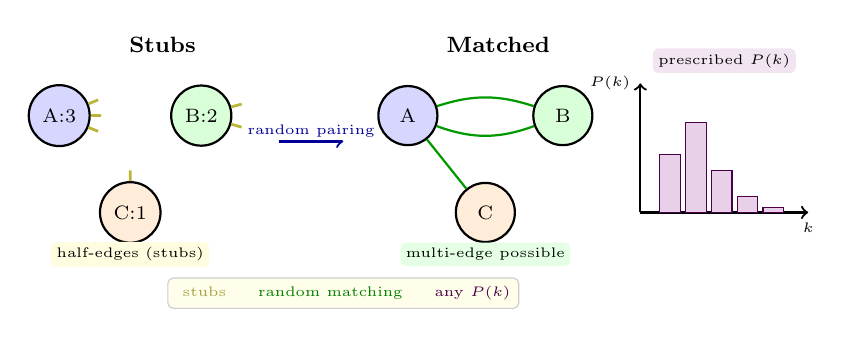
\begin{tikzpicture}[scale=0.82,every node/.style={font=\scriptsize}]
% stubs before matching
\begin{scope}
\node[font=\footnotesize\bfseries] at (1.6,2.6) {Stubs};
\node[circle,draw,thick,fill=blue!16,minimum size=0.75cm] (a) at (0,1.5) {A:3};
\foreach \ang in {-22,0,22} \draw[thick,yellow!70!black,line width=1.0pt] (a) -- ++(\ang:0.65);
\node[circle,draw,thick,fill=green!15,minimum size=0.75cm] (b) at (2.2,1.5) {B:2};
\foreach \ang in {-16,16} \draw[thick,yellow!70!black,line width=1.0pt] (b) -- ++(\ang:0.65);
\node[circle,draw,thick,fill=orange!15,minimum size=0.75cm] (c) at (1.1,0) {C:1};
\draw[thick,yellow!70!black,line width=1.0pt] (c) -- ++(90:0.65);
\node[font=\tiny,fill=yellow!12,rounded corners=2pt,inner sep=2pt] at (1.1,-0.65) {half-edges (stubs)};
\end{scope}
\draw[->,thick,blue!60!black] (3.4,1.1)--(4.4,1.1) node[midway,above,font=\tiny,fill=white,inner sep=1pt] {random pairing};
% matched
\begin{scope}[xshift=5.4cm]
\node[font=\footnotesize\bfseries] at (1.4,2.6) {Matched};
\node[circle,draw,thick,fill=blue!16,minimum size=0.75cm] (a2) at (0,1.5) {A};
\node[circle,draw,thick,fill=green!15,minimum size=0.75cm] (b2) at (2.4,1.5) {B};
\node[circle,draw,thick,fill=orange!15,minimum size=0.75cm] (c2) at (1.2,0) {C};
\draw[thick,green!60!black] (a2) to[bend left=18] (b2);
\draw[thick,green!60!black] (a2) to[bend right=20] (b2);
\draw[thick,green!60!black] (a2)--(c2);
\node[font=\tiny,fill=green!10,rounded corners=2pt,inner sep=2pt] at (1.2,-0.65) {multi-edge possible};
\end{scope}
% degree histogram
\begin{scope}[xshift=9.0cm]
\draw[->,thick] (0,0)--(2.6,0) node[below,font=\tiny] {$k$};
\draw[->,thick] (0,0)--(0,2.0) node[left,font=\tiny] {$P(k)$};
\foreach \x/\h in {0.3/0.9,0.7/1.4,1.1/0.65,1.5/0.25,1.9/0.08} \draw[fill=violet!18,draw=violet!60!black] (\x,0) rectangle +(0.32,\h);
\node[font=\tiny,fill=violet!10,rounded corners=2pt,inner sep=2pt] at (1.3,2.35) {prescribed $P(k)$};
\end{scope}
\node[font=\tiny,draw=gray!40,fill=yellow!8,rounded corners=2pt,inner sep=3pt] at (4.4,-1.25) {\textcolor{yellow!60!black}{$\blacksquare$ stubs} \quad \textcolor{green!50!black}{$\blacksquare$ random matching} \quad \textcolor{violet!60!black}{$\blacksquare$ any $P(k)$}};
\end{tikzpicture}
\caption{Configuration model: create $k_i$ stubs per node (left), pair uniformly (centre) to realise any prescribed degree distribution (right). For sparse graphs self-loops and multi-edges are $O(1/n)$.}
\label{fig:config-stubs}
\end{figure}

A key null-model use: compute modularity or clustering on the real graph, then compare to the configuration ensemble with the same degrees. If the real $Q$ far exceeds the random $Q$, communities are significant.

% ============================================================
\section{Watts--Strogatz Small-World}
\label{sec:ws}
\paragraph{Intuition.} ER has short paths ($\sim\log n$) but negligible clustering ($C\sim\langle k\rangle/n$). A ring lattice has high clustering ($C\approx3/4$ for $k=4$) but long paths ($\sim n/2k$). Real networks have \emph{both}: e.g.\ social nets are clustered yet six degrees apart. Watts and Strogatz rewired a lattice slightly to get both.

\begin{definition}[Watts--Strogatz model]\label{def:ws}
Start with a ring of $n$ nodes, each linked to $k/2$ neighbours on each side ($k$ even). For each edge $(i,j)$, with probability $p$ rewire it to $(i,\ell)$ where $\ell$ is random (avoid duplicates/self-loops). $p=0$ is the lattice; $p=1$ is random-like; intermediate $p\sim0.01$--$0.1$ gives high $C$ and low $L$---the small-world regime.
\end{definition}

\begin{figure}[h]\centering
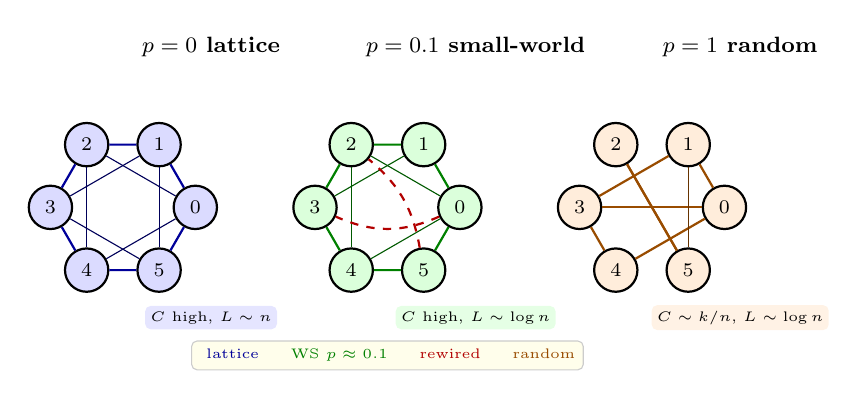
\begin{tikzpicture}[scale=0.80,every node/.style={font=\scriptsize}]
\begin{scope}
\node[font=\footnotesize\bfseries] at (1.4,2.55) {$p=0$ lattice};
\foreach \i in {0,...,5} {\node[circle,draw,thick,fill=blue!14,minimum size=0.55cm] (n\i) at (60*\i:1.15) {\i};}
\foreach \i in {0,...,5} {\pgfmathtruncatemacro{\j}{mod(\i+1,6)} \draw[thick,blue!60!black] (n\i)--(n\j);
\pgfmathtruncatemacro{\k}{mod(\i+2,6)} \draw[thin,blue!35!black] (n\i)--(n\k);}
\node[font=\tiny,fill=blue!10,rounded corners=2pt,inner sep=2pt] at (1.4,-1.75) {$C$ high, $L\sim n$};
\end{scope}
\begin{scope}[xshift=4.2cm]
\node[font=\footnotesize\bfseries] at (1.4,2.55) {$p=0.1$ small-world};
\foreach \i in {0,...,5} {\node[circle,draw,thick,fill=green!14,minimum size=0.55cm] (m\i) at (60*\i:1.15) {\i};}
\foreach \i in {0,...,5} {\pgfmathtruncatemacro{\j}{mod(\i+1,6)} \draw[thick,green!50!black] (m\i)--(m\j);}
\foreach \i in {0,1,2,4} {\pgfmathtruncatemacro{\k}{mod(\i+2,6)} \draw[thin,green!35!black] (m\i)--(m\k);}
\draw[thick,red!70!black,dashed] (m0) to[bend left=24] (m3);
\draw[thick,red!70!black,dashed] (m5) to[bend right=20] (m2);
\node[font=\tiny,fill=green!10,rounded corners=2pt,inner sep=2pt] at (1.4,-1.75) {$C$ high, $L\sim\log n$};
\end{scope}
\begin{scope}[xshift=8.4cm]
\node[font=\footnotesize\bfseries] at (1.4,2.55) {$p=1$ random};
\foreach \i in {0,...,5} {\node[circle,draw,thick,fill=orange!14,minimum size=0.55cm] (q\i) at (60*\i:1.15) {\i};}
\draw[thick,orange!60!black] (q0)--(q1); \draw[thick,orange!60!black] (q1)--(q3); \draw[thick,orange!60!black] (q2)--(q5);
\draw[thick,orange!60!black] (q3)--(q4); \draw[thick,orange!60!black] (q4)--(q0); \draw[thick,orange!60!black] (q5)--(q2);
\draw[thick,orange!60!black] (q0)--(q3); \draw[thin,orange!40!black] (q1)--(q5);
\node[font=\tiny,fill=orange!10,rounded corners=2pt,inner sep=2pt] at (1.4,-1.75) {$C\sim k/n$, $L\sim\log n$};
\end{scope}
\node[font=\tiny,draw=gray!40,fill=yellow!8,rounded corners=2pt,inner sep=3pt] at (4.2,-2.35) {\textcolor{blue!60!black}{$\blacksquare$ lattice} \quad \textcolor{green!50!black}{$\blacksquare$ WS $p\approx0.1$} \quad \textcolor{red!70!black}{$\blacksquare$ rewired} \quad \textcolor{orange!60!black}{$\blacksquare$ random}};
\end{tikzpicture}
\caption{Watts--Strogatz rewiring. A lattice ($p=0$) has high clustering but long paths. Rewiring a few edges (red dashed, $p\approx0.1$) drops $L$ dramatically while $C$ stays high---the small-world. Full rewiring ($p=1$) randomises.}
\label{fig:ws-rewiring}
\end{figure}

\begin{lstlisting}[language=Python, caption={ER giant-component hunt: sweep $p$ and track largest component.}, label={lst:er-giant}]
import networkx as nx
import numpy as np

def giant_fraction(n, p, trials=20):
    fracs = []
    for _ in range(trials):
        G = nx.erdos_renyi_graph(n, p)
        largest = max(len(c) for c in nx.connected_components(G)) if G else 0
        fracs.append(largest / n)
    return np.mean(fracs)

for p in [0.005, 0.01, 0.02, 0.05]:
    print(f"p={p:.3f} <k>={p*99:.1f} S~{giant_fraction(100,p):.2f}")
# Watch S jump near p=1/n=0.01
\end{lstlisting}

\begin{lstlisting}[language=Python, caption={Configuration and Watts--Strogatz: prescribed degrees and the small-world trade-off.}, label={lst:config-ws}]
import networkx as nx

# Configuration model: power-law-ish degree sequence
deg_seq = [5,4,3,3,2,2,1,1,1,1]
G_cfg = nx.configuration_model(deg_seq, seed=0)
G_cfg = nx.Graph(G_cfg)  # remove multi-edges
G_cfg.remove_edges_from(nx.selfloop_edges(G_cfg))
print("cfg degrees:", sorted([d for _,d in G_cfg.degree()], reverse=True))

# WS small-world sweep
for p in [0, 0.05, 0.5, 1.0]:
    WS = nx.watts_strogatz_graph(30, 4, p, seed=1)
    print(f"p={p:.2f} C={nx.average_clustering(WS):.3f}"
          f" L={nx.average_shortest_path_length(WS):.2f}")
\end{lstlisting}

% ============================================================
\section{Chapter Notes}
Erd\H{o}s and R\'enyi (1959, 1960) founded random-graph theory; the phase-transition picture via branching processes was clarified by Bollob\'as (2001). The configuration model was systematised by Bender--Canfield and Molloy--Reed. Watts and Strogatz (1998, \emph{Nature}) sparked the modern small-world revival; Kleinberg (2000) added navigability. Always state whether $G(n,p)$ or $G(n,M)$ is meant---their fluctuations differ but typical properties agree.

% ============================================================
\section{Exercises}
\label{sec:ch04-exercises}
\begin{enumerate}[label=E4.\arabic*, leftmargin=*, itemsep=0.8em]
    \item \textbf{ER degree check.} For $G(200, p=0.015)$ compute $\langle k\rangle$, the Poisson prediction $P(0)$, and expected number of isolated nodes. Simulate 30 trials and compare.
    \item \textbf{Threshold estimation.} Fix $n=500$, sweep $p$ from $0$ to $0.01$ (step $0.001$), and estimate giant-component fraction $S/n$ (average 20 trials). Plot and identify where $S$ lifts off---compare to $1/n$.
    \item \textbf{Configuration model multi-edges.} Generate a configuration model with degrees $[8,8,1,1,1,1,1,1]$ ($n=8$). How often do multi-edges or self-loops appear in 100 trials? Why does a hub-heavy sequence increase collision probability?
    \item \textbf{WS trade-off.} For $n=100$, $k=6$, sweep $p\in\{0,0.01,0.05,0.1,0.5,1\}$ and measure $C(p)/C(0)$ and $L(p)/L(0)$. At which $p$ does $L$ drop to half while $C$ stays above $0.5\,C(0)$? This is the small-world window.
    \item \textbf{Null-model test.} Compute modularity $Q$ of the karate club under Louvain. Generate 30 configuration-model randomisations (same degree sequence) and compute their $Q$ values. Is the real $Q$ significant (how many standard deviations above the random mean)?
\end{enumerate}
% End of Chapter 4
